\documentclass[10pt,a4paper]{article}
\usepackage{listings}
\usepackage[utf8]{inputenc}
\usepackage{color}
\usepackage[francais]{babel}
\usepackage[T1]{fontenc}
\usepackage{graphicx}
\usepackage[export]{adjustbox}
\bibliographystyle{ieeetr}
\author{Ali CHERIFI}
\title{Rapport de stage de licence\\Résumé vidéo et vidéo 3D anaglyphe et side-by-side}
\begin{document}
\maketitle
\newpage
\tableofcontents
\newpage
\section{Introduction}
Le relief de la vision humaine provient de la différence de perception entre les deux yeux. La stéréoscopie rassemble toutes les différentes méthodes permettant de reconstruire cet effet à partir d'objets 2D
observés soit à travers un instrument d'optique ou alors à partir de deux photographies prises avec un décalage.
La stéréoscopie est un domaine qui a interessé l'homme depuis longtemps. En effet, ce principe a été imaginé par Charles Wheatstone\cite{stereoscopie} (physicien et inventeur anglais) en 1832.
Le premier appareil créant l'effet stéréoscopique a vu le jour en 1843 par David Brewster (physicien et inventeur écossais). Cet appareil ne servait alors qu'à observer deux dessins.
Cet appareil monta en popularité avec l'apparition des travaux sur la photographie. Il était constitué de deux prismes comportant chacun des faces convexes. Cela permettait à chaque oculaire de
produire à la fois l'effet d'un prisme et d'une lentille. L'impression de relief était donc observable sur deux photographies donc le centre de la deuxième est décalé de quelques centimètres.

\begin{figure}[!h]
\center
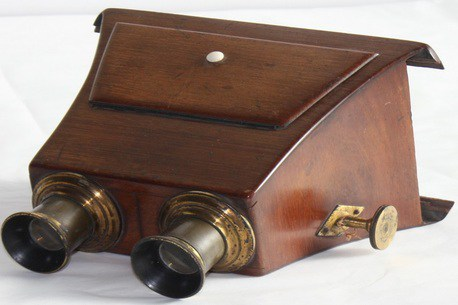
\includegraphics[scale = 0.5]{brewer.jpg}
\caption{Stéréoscope de Brewer\cite{brewster}.}
\end{figure}

Un procédé voisin mais néanmoins différent est celui de l'anaglyphe. Ce procédé sera décrit plus en détail dans la section\ref{anasbs}.
Actuellement les dispositifs les plus populaires s'inspirent du stéréoscope de Brewer pour reconstruire le relief comme le fait l'Oculus Rift ou l'HTC Vive. La technologie side-by-side est utilisée ici et
sera vu en détail dans la section \ref{anasbs}.

Ces deux procédés ont très vite été adaptés aux vidéos afin de rendre les films plus vivants et réels et ainsi augmenter l'immersion.
A l'heure actuelle tous ces procédés utilisent 2 photographies ou vidéos prise avec un point de vue différents.  Le rendu du relief est alors très convaincant car très proche de la réalité.
Cependant, se procurer deux caméras ou appareils photos est très onéreux et n'est pas à la portée de tout le monde. Le but ici sera donc de réfléchir et de trouver un moyen de produire
cette stéréoscopie à partir d'une seule source vidéo ou d'une seule photographie tout en obtenant un relief le plus convaincant possible. Le résultat ne sera cependant jamais le même qu'avec deux images,
la perspective étant fixe à partir d'une seule source. Lors d'une prise avec 2 appareils, certains éléments sortent du cadre de la photo tandis que d'autres y entre. La quantité
d'informations présente sur une image est fixe. La translation qui se fera pour produire le décalage entre les deux yeux constituera alors une perte d'informations sans aucun gain.

Le but ici est donc d'automatiser le processus de création d'une vidéo stéréoscopique anaglyphe et side-by-side à partir d'une seule source vidéo tout ceci en JAVA.

\section{Laboratoire d'accueil}

Mon stage est effectué au sein du LaBRI, le Laboratoire Bordelais de Recherche en Informatique. Le LaBRI est associé au CNRS, à l'Université de Bordeaux ainsi qu'à l'INP (Institut Polytechnique de Bordeaux)\cite{labri}.
Le LaBRI compte environ 300 personnes dont 113 enseignants et chercheurs de l'Université de Bordeaux et de L'INP et 37 chercheurs répartis entre L'INRIA (Institut National de Recherche en Informatique et en Automatique) et le CNRS. Le LaBRI compte également 140 doctorants, post-doctorants et ingénieurs contractuels.
Six équipes existent au sein du LaBRI axant leur recherche sur différents domaines. Les équipes sont les suivantes :\\

\begin{itemize}
\item Combinatoire et Algorithmie
\item Méthodes Formelles
\item Modèles et Algorithmes pour la Bioinformatique et la Visualisation d'informations
\item Programmation, Réseaux et Systèmes
\item Supports et Algorithmes pour les Applications Numériques Hautes performances.
\item Image et Son\\
\end{itemize}

Mon stage s'effectuera au sein de l'équipe Image et Son.

\section{Etat de l'art et matériel existant}
\subsection{Résumé vidéo}
Le résumé vidéo peut aussi être appelé "Movie Barcode". Il permet de faire ressortir la couleur générale d'un film ou d'une vidéo. En récupérant la bande du milieu de chaque image et en concaténant tout cela pour
tout le film, on obtient une image très similaire à un code barre représentant l'ambiance générale de la vidéo.
Il existe un logiciel disponible réalisant ce traitement nommé "Movie Barcode Generator". Le logiciel est écrit en C\# et ses sources sont disponibles à tous\cite{barcode}. L'auteur du logiciel accepte la vente des résultats produit par son logiciel.

SCREEN BARCODE

\subsection{Anaglyphe et side-by-side}
\label{anasbs}
Actuellement, le vidéo 3D par anaglyphe propose deux méthodes majeures, un algorithme simple et la méthode de Dubois.
Le premier algorithme consiste à séparer et extraire les canaux RGB d'une image 2D et d'en faire une image 3D. Le principe réside dans le filtrage des couleurs par l'œil devant lequel se trouve un filtre.
Chaque œil ayant un filtre différent, il ne perçoit que les couleurs que le filtre laisse passer. Actuellement, le filtre le plus répandu est le filtre rouge/cyan.
Il suffit donc dans le cas de cet algorithme, d'extraire le canal rouge de l'image et d'en générer un nouvelle. Ensuite il faut à partir de l'image source créer une nouvelle image à partir du mélange des canaux bleu et vert.
On obtient ainsi deux images, une cyan et l'autre rouge. Il faut ensuite les superposer en leur appliquant un décalage(voir figure \ref{anaglyphe}.\newline

\begin{figure}[!h]
\center
\includegraphics[scale = 0.5]{anaglyphe.jpg}
\caption{Image anaglyphée.}
\label{anaglyphe}
\end{figure}

Éric Dubois est ingénieur et chercheur à l'Université d'Ottawa au Canada\cite{duboisbio}. Ses travaux sur la stéréoscopie commencent lors d'un projet en collaboration avec IMAX\footnote{Entreprise ayant mis au point le format IMAX, dix fois plus large que les tailles d'écrans de cinéma classique.}. Éric Dubois propose de modifier les couleurs de l'image avant de lui appliquer l'algorithme vu précédemment.
En effet, afin de générer des couleurs anaglyphe les plus proche possible de l'originale, Éric Dubois tiens compte de la sensibilité spectrale de l'œil humain,
le spectre d'absorption des filtre des lunettes et de la densité du spectre des moniteurs\cite{dubois}.
Éric Dubois a alors pu en déduire une matrice à appliquer sur l'image originale permettant un effet 3D amélioré et la quasi-disparition des images fantômes qui sont des images résultant d'une superposition mal effectuée. Le résultat obtenu est donc similaire à un anaglyphe classique (cf. \ref{anaglyphe}) aquel se rajjoute une légère modification des couleurs.
Le logiciel open-source Gimpel3D permet de faire de l'anaglyphe à partir d'images seulement et ne propose pas la méthode d'Éric Dubois. Nombre de logiciels payant existent et propose de réaliser des vidéos 3D anaglyphe suivant l'algorithme basique comme par exemple DVDFab 9 ou  3D Video Converter.\newline

En ce qui concerne le side-by-side, le principe est de reproduire la distinction entre l'œil droit et l'œil gauche à travers une vidéo comportant les mêmes images aux mêmes instants mais très légèrement décalés(voir figure \ref{sbs}). On observe donc des éléments tronqués où manquants entre les deux images.
Il existe à l'heure actuelle beaucoup de logiciels qui proposent de faire ceci mais uniquement à partir de deux vidéos enregistrés préalablement avec le décalage.
Un seul logiciel exécute ce traitement avec une seule vidéo et il s'agit de DVDFab 9. Il est cependant payant et il n'existe aucun autre logiciel gratuit ou open-source réalisant ce traitement.

\begin{figure}[!h]
\center
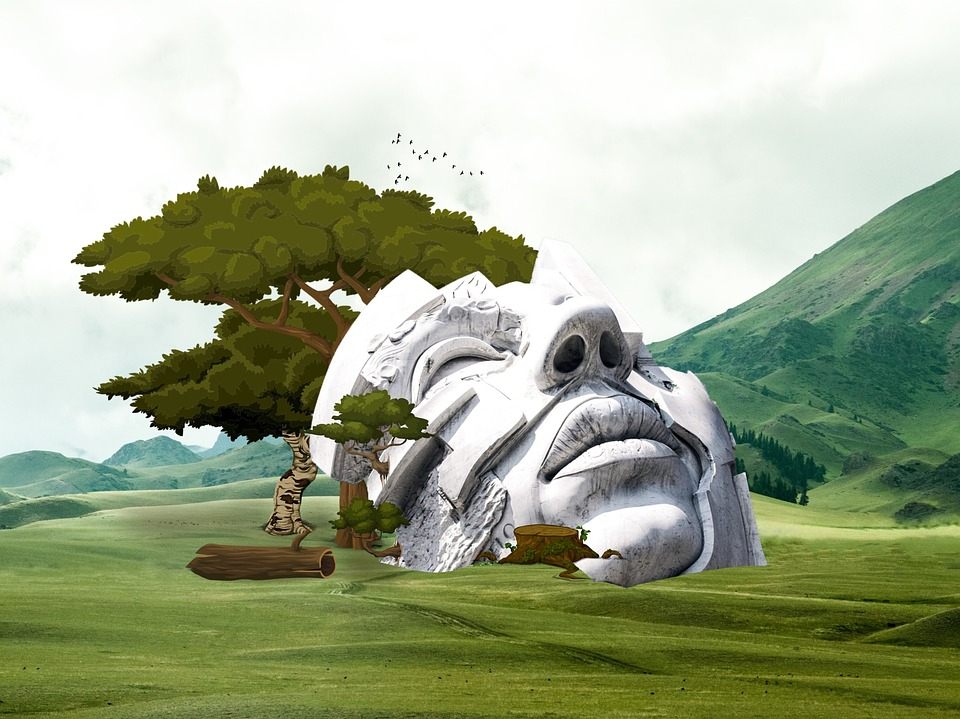
\includegraphics[scale = 0.3]{sbs.jpg}
\caption{Image Side-by-side.}
\label{sbs}
\end{figure}

\subsection{Les flux vidéos en JAVA}

Très peu de bibliothèques manipulant des vidéos existent en JAVA. Au fil des recherches, la première bibliothèque que j'ai pu rencontrer est JAVACV\cite{javacv}, qui est un wrapper\footnote{Englobage d'un élément déjà existant
afin de simplifier son utilisation.} autour d'OpenCV. Cependant, les performances de JAVACV sont encore aujourd'hui sujet de débat.\\

J'ai donc préféré m'orienter vers des bibliothèques multimédias. J'ai trouvé par la suite la bibliothèque nommée Xuggler\cite{xuggler} qui est un wrapper autour de
ffmpeg\footnote{Collection de logiciel libre permettant le traitement de flux audio et vidéos.} pour JAVA. Après quelques essais en ligne de commande de ce qui était offert
par ffmpeg (extraction des frames d'une vidéo, grands nombre de formats décodables,etc...), j'ai donc voulu essayer Xuggler. Malheureusement, cette bibliothèque n'est plus maintenue à jour, en effet le dernier
commit GitHub date de 2014\cite{xugglergit}. En recherchant d'autres wrapper autour de ffmpeg j'ai finalement pu tomber sur la bibliothèque OpenIMAJ\cite{openimaj} et c'est celle-ci que j'utiliserais.\\

Afin de traiter les flux vidéos et de faire le traitement nécessaire sur les images tirées des vidéos, je me servirais de  la bibliothèque OpenImaj car multimédia, et maintenue à jour.
Cette bibliothèque présente de nombreux avantages. Tout d'abord elle est
disponible via un dépot Maven sous forme de modules\cite{openimajmvn}. On peut donc récupérer uniquement les éléments de la bibliothèque
les plus pertinents. J'ai donc besoin ici des modules de décodage vidéo et de son, du module de traitement d'images
et du module gérant les entrées/sorties.
Comme dit précédemment, OpenIMAJ est un wrapper ffmpeg. On aura donc l'avantage ici de pouvoir décoder les formats vidéos
les plus utilisés, causant alors très peu de problèmes de compatibilité dans notre
programme.\\

L'encodage quant à lui est par contre beaucoup plus restreint. Cela ne nous empêchera pas de produire
le fichier de sortie dans les formats les plus courants c'est-à-dire MP4, AVI ou MKV.
En ce qui concerne l'image, notre programme donnera en sortie une image au format PNG afin d'éviter la perte de donnée et
pour pouvoir l'exporter facilement sur le web.

Le son des vidéos sera quant devrait être restitué tel qu'il l'était sur le fichier source.

\section{Cahier des charges et architecture}

\subsection{Cahier des charges}

Besoins fonctionnels :\newline
\begin{itemize}
\item S'affiche sous forme de fenêtre.
\item Choisir le fichier à traiter.
\item Préciser si la vidéo est décodable par le logiciel ou non. Si non, précisez les formats acceptés.
\item choix du mode de traitement et de l'algorithme (pour l'anaglyphe choisir entre l'algorithme classique ou la méthode
de Dubois).
\item Effectuer le traitement à l'aide d'un bouton.
\item Montrer l'avancement du traitement.
\item Sauvegarder le fichier sous le nom que l'on veut.
\item pré-visualiser la vidéo sélectionnée\newline
\end{itemize}

Non fonctionnels :\newline
\begin{itemize}
\item Le logiciel doit être rapide. Le traitement doit s'effectuer dans le pire des cas dans le temps de la vidéo.
\item Fidélité. Le logiciel ne doit pas détériorer la qualité de la vidéo originelle.
pdf.\newline
\end{itemize}

\subsection{Architecture}

Mon projet sera découpé en différents paquetages, correspondant aux éléments composant le logiciel: traitements, boutons, tests, exceptions et utilitaires (voir figure \ref{arbo}).

\begin{figure}[!h]
\center
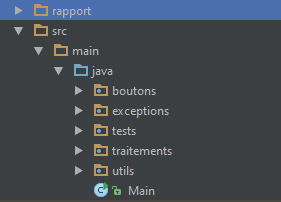
\includegraphics[scale = 1]{tree.PNG}
\caption{Arborescence du projet.}
\label{arbo}
\end{figure}

Mon application comprendra une interface simple composé d'un menu permettant de choisir les traitements. En dessous de ce menu se trouveront deux champs permettant de renseigner le fichier vidéo à traiter ainsi que de préciser le fichier de sortie.

SCREEN GLOBAL

Le logiciel comporte deux exceptions. Une de ces exceptions \textit{VideoNonSupporte} est chargée de vérifier si le fichier sélectionné en entrée est supporté par la bibliothèque ou s'il s'agit bien d'une vidéo. OpenImaj ne dispose pas de méthode permettant de vérifier si la vidéo est décodable, l'exception vérifié donc si le fichier sélectionné à un nombre de frames différent de zéro. Une vidéo non décodable ou un fichier quelconque aura un nombre de frame égal à -1 (valeur par défaut dans OpenIMAJ). Lever cette exception interrompt la suite du chargement de la vidéo, elle n'est pas prise en compte.

La deuxième exception se charge de vérifier si un fichier de destination a été précisé. Lors du lancement d'un traitement, si aucun fichier de destination n'est precisé, le traitement ne se lance pas et une boîte de dialogue informe l'utilisateur qu'il faut rentrer une fichier de destination.


Lors de l'appui sur le bouton pour charger une vidéo, c'est la classe ChargerVideo qui est appellée.
Le constructeur de cette classe prend en paramètre un JTextArea et un JPanel. Le JTextArea permet de faire apparaitre le chemin de la vidéo sélectionnée. Le JPanel quant à lui est le conteneur permettant de centrer l'apparation de l'exception \textit{VideoNonSupporte} si le fichier sélectionné ne peut être décodé.

Lors de l'appui sur le bouton, un JFileChooser est lancé puis passé à la méthode \textit{chargerVideo(JFileChooser fichier)}.
Cette méthode se charge d'ouvrir la fenêtre de sélection du fichier puis créé 1 flux audio pour la vidéo sélectionnée ainsi qu'un affichage pour visualiser la vidéo. Cette méthode lance l'exception \textit{VideoNonSupporte} si la vidéo n'est pas décodable.
2 flux vidéos sont également créés, l'un servant à être envoyé au traitement et l'autre servant au lecteur vidéo. Il est
nécessaire de charger deux fois la vidéo pour effacer le lien affichage/traitement. En effet, si la vidéo traitée est la même pour l'affichage, regarder la vidéo jusqu'à par exemple la moitié fera commencer le traitement sélectionné à la moitié de la vidéo.

Le bouton permettant de choisir le fichier de destination fait appel à la classe \textit{Sauvegarder} qui elle ne prends en paramètre que le JTextArea pour afficher le chemin du fichier de sortie. Elle fonctionne de manière similaire à la classe de chargement.

Une fois ces deux renseignements apportés, l'utilisateur peut alors utiliser le menu des traitements pour choisir lequel appliquer sur sa vidéo. A l'exception du movie barcode, tous les traitements se lance directement en cliquant sur leur nom. L'utilisateur verra alors un JOptionPane s'afficher, lui indiquant que le tratiement est en cours. Tous ces traitements s'exécute aux seins de threads qui permettent à la fenêtre de s'afficher et au traitement de s'éxecuter en simultané. Si l'utilisateur choisit par exmple l'anaglyphe, un click provoque un appel à la classe \textit{ListenerAnaglyphe} qui implémente un \textit{ActionListener}. Cette classe instancie un textit{ThreadAnaglyphe} et le lance. Cette dernière hérite de textit{Thread} et lance la méthode textit{Traitement.anaglyphe()}. 

SCREEN FENETRE TRAITEMENT

Concernant le movie barcode, un click sur dans le menu affiche une fenêtre permettant de saisir les options voulues c'est-à-dire la largeur de l'image et la taille de la bande centrale à récupérer. Ces données sont sauvegarder dans la classe textit{OptionsBarcode} implémentée en static. Cette fenêtre comporte deux JTextArea, un pour entrer la largeur de l'image et l'autre pour entrer la taille de la bande. Deux clicks sur deux boutons textit{Ok} sont nécessaires pour sauvegarder les valeurs via les méthodes textit{OptionsBarcode.setLargeur} et textit{OptionsBarcode.setTailleBande}. Un click sur le bouton textit{Valider} permet de lancer le traitement via les threads de manière similaire aux autres traitements.

SCREEN OPTIONS BARCODE

Une fois le traitement selectionné, un JOptionPane indique que le traitement est en cours via la classe textit{ThreadEnCours} lancé au début du traitement. Ce JOptionPane est ensuite détruit en fin de traitement et remplacé par un autre indiquant la fin du traitement.

SCREEN



\section{Implémentation}

La première chose que j'ai eu à réaliser a été de créer le projet Maven\footnote{Outil pour la gestion automatique des projets.}. OpenIMAJ étant disponible via Maven,
j'ai eu a rédiger le fichier pom.xml permettant de récupérer les modules nécessaires. Le fichier es découpé en section à l'aide de balises de façon similaire à l'HTML. Il faut en début de fichier,
déclarer le projet, sa version, ainsi que les dépôts distants où récupérer les modules. \newpage

\lstinputlisting[language=XML, firstline=1, lastline=17,frame=tb,columns=fixed,keywordstyle=\color{blue},breaklines=true,keepspaces,caption = En-tête du ficher pom.xml.]{../pom.xml}

~~\\
Il faut ensuite ouvrir la balise des dépendances et inscrire chaque dépendance que l'on trouve sur le site du dépôt Maven de OpenIMAJ\footnote{https://mvnrepository.com/artifact/org.openimaj}.\\

\lstinputlisting[language=XML, firstline=19, lastline=32,frame=tb,columns=fixed,keywordstyle=\color{blue},keepspaces,breaklines=true, caption = Dépendances nécessaires.]{../pom.xml}
~~\\


Je commence ensuite l'élaboration des algorithmes. J'ai donc commencé par l'écriture de l'algorithme du movie barcode.
\subsection{Movie Barcode}

Le movie barcode doit, pour restaurer la couleur d'une image, récupérer la bande centrale de chaque frame de la vidéo. Je suis donc passé par l'écriture de la méthode \textit{getBandeCentrale(MBFImage source)},
qui prends en paramètre une frame et retourne la bande centrale de cette frame. L'algorithme se place au milieu de l'image et la parcours de la manière suivante : $milieu - tailleBande /2$ jusqu'à $milieu + tailleBande /2$. Une nouvelle image est créée de hauteur similaire à l'image source et de largeur de la taille de  la bande. Dans cette image sont placés la couleur des pixels extraits de l'image source. La méthode retourne ensuite cette image.

Une fois ceci fait, l'algorithme du barcode se contente de concaténer toutes les bandes centrales dans une seule image finale. Le programme ne parcours cependant que les keyframes de la vidéo, les keyframes étant les seules images codées complètement dans une vidéo, les autres étant calculées à partir des précédentes
(P-frame) ou des suivantes (B-frame)\footnote{http://www.dacast.com/blog/what-is-a-key-frame-for-video/}. OpenIMAJ dispose d'une méthode permettant de dessiner une image dans une autre. Comme la hauteur a été renseignée par l'utilisateur 


\subsection{Side-by-side}

Concernant le side-by-side, c'est en étudiant des vidéos produites avec deux sources que j'ai pu me faire une idée de l'algorithme à mettre en œuvre. Outre la perspective changeante,
ce qui change le plus sur une vidéo side-by-side est ce qui est perçu par les deux caméras. J'ai donc décidé de tronquer mon image source. L'image censée reproduire l'œil gauche sera tronquée sur la droite.
Il manquera donc une partie sur l'image de droite. Quant à l'image de droite, elle sera tronquée sur la gauche.  Nous aurons donc ici deux images qui mises côte à côte et observées avec le dispositif adéquat,
donneront une image complète.
Ce découpage passe donc par l'appel de deux méthodes \textit{decouperImageGauche()} et \textit{decouperImageDroite()} qui se chargeront de découper les images.

\lstinputlisting[language=JAVA, firstline=363, lastline=383,frame=tb,columns=fixed,keywordstyle=\color{blue},keepspaces, breaklines=true,  basicstyle=\footnotesize, caption = Découpage de l'image gauche.]{../src/main/java/traitements/Traitement.java}
~~\\

Une fois ce découpage effectué il faut alors assembler les deux images ce que fait la méthode \textit{sideBySideImage(MBFImage source)}.
Il faut donc créer une image de taille $(largeurImageSource - ESPACEMENT) * 2$. Ici ESPACEMENT, correspond à l'écart moyen entre les deux yeux.
Les deux images font donc la même taille c'est-à-dire $largeurImageSource - ESPACEMENT$. On peut donc avoir une image finale où la résolution par œil sera la même que l'image source. L'image
finale fait donc deux fois cette taille ci.

Il reste donc une fois cette image crée à l'ajouter dans une vidéo de sortie. C'est ce que fait la méthode \textit{sideBySide()}.

\lstinputlisting[language=JAVA, firstline=246, lastline=270,frame=tb,columns=fixed,keywordstyle=\color{blue},keepspaces, breaklines=true,  basicstyle=\footnotesize, caption = Création de la vidéo.]{../src/main/java/traitements/Traitement.java}

\subsection{Anaglyphe classique et méthode de Dubois}

L'algorithme d'anaglyphe récupère toutes les frames d'une vidéo et leur applique à chacune l'effet d'anaglyphe. Cela passe donc par la méthode \textit{anaglypheImage(MBFImage source, int largeur, int hauteur)}
qui récupère l'image en paramètre et retourne la même image anaglyphée. Le passage en paramètre de la hauteur et de la largeur évite de recalculer ces deux données à chaque appel de la méthode.


l'algorithme créant la vidéo anaglyphée consiste à envoyer toutes les frames àa cette méthode et à reconstruire une vidéo à partir de ces frames à l'aide de l'objet
\textit{XuggleVideoWriter}. Le format de sortie de la vidéo est spécifié par le format d'entrée.

En ce qui concerne la méthode de Dubois, j'ai utilisé la matrice moyenne élaborée pour modifier les couleurs de l'image. Éric Dubois travaille toujours avec deux images, donnant un effet de relief plus
convaincant. J'ai donc décidé d'appliquer le même tronquage sur mon image source que celui réalisé sur le side-by-side afin d'obtenir deux images différentes en termes d'informations. Je peux ensuite
appliquer la matrice sur les pixels des deux images. Cela me donne donc une image anaglyphée présentant une effet 3D plus convaincant que l'algorithme classique.

\section{Phase de test}

Le projet reposant sur la vision stéréoscopique et donc la reconstruction par le cerveau de la perpective, il va être ici compliqué de tester à l'aide d'algorithmes les images obtenues. Cependant, il est possible de tester automatiquement le movie barcode ainsi que le découpage des images qui a lieu lors du side-by-side ou de l'anaglyphe de Dubois. 

\subsection{Tests sur le movie barcode}

L'essentiel de l'algortihme repose sur la récupération de la bande centrale de l'image. J'ai donc créée une méthode qui me créé une image noir avec une bande centrale rouge. Je fais ensuite appel à la méthode textit{getBandeCentrale(MBFImage image, int tailleBande)} pour récupérer la bande rouge. Afin de vérifier si le découpage est correct, mon algorithme parcourt la bande et vérifie que tous les pixels sont bien rouges. 

En ce qui concerne le découpage des images, je dispose de deux méthodes créant des images spécifiques pour les tests. Sur une même vue observée par l'oeil humain, l'image perçue par l'oeil gauche est tronquée sur la droite et inversement pour l'oeil droit. La méthode textit{creationImgGauche()} créée donc une image noire avec une bande rouge sur la droite. La méthode textit{creationImgDroite()} crée quant à elle une image avec une bande rouge sur la gauche.

\section{Conclusion}

L'échéance arrivée, le programme remplit ses fonctions. Il est capable d'ouvrir une vidéo et d'effectuer le résumé vidéo, l'anaglyphe classique et selon la méthode de Dubois ainsi que le side-by-side. Le programme prévient l'utilisateur si la vidéo est décodable ou non et si l'utilisateur tente des opérations sans fichier source ou sans fichier de destination.

Les traitements sont réalisable cependant excepté le résumé vidéo, les autres traitements ne sont pas réalisé en 1/1 (c'est-à-dire dans le temps de la vidéo). En effet les traitements sont deux voire trois fois plus long que la vidéo. En regardant de plus près le code source d'OpenIMAJ, j'ai pu voir que les pixels sont codés par des flottants entre  0 et 1. Cela pourrait donc induire des temps de calculs plus longs afin de manipuler les nuances de couleurs.

La bibliothèque OpenIMAJ présente également des problèmes de compatibilité entre les différentes plates-formes. Le projet ayant été realisé majoritairement sous Linux, lors d'un test sur une plate-forme Windows, la bibliothèque est incapable d'ouvrir une vidéo situé sur l'ordinateur.

La bibliothèque n'est pas capable de restituer du son. En effet, un flux audio petu être ouvert à partir d'une vidéo mais OpenIMAJ ne peut pas le lier à un flux vidéo. Tous les traitements donnent donc pour résultat une vidéo sans son. De plus, lors de l'ouverture de l'audio et de la vidéo lors de la pré-visualisation, les deux se lancent automatiquement. Il est possible de mettre en pause la vidéo mais pas l'audio. L'audio se lance donc sans la vidéo, il est alors nécessaire de lancer la vidéo puis de mettre la lecture sur pause pour que les deux s'arrêtent.

Avec plus de temps, j'aurais pu optimiser mes traitements afin d'atteindre un temps de rendu égal à celui de la vidéo source. J'aurais également pu chercher une bibliothèque gérant mieux le son qu'OpenIMAJ et ne garder OpenIMAJ que pour la gestion de la vidéo et le traitements des images.





\newpage
\bibliography{biblio}


\end{document}